%%
%% This is file `sigconf.tex',
%% generated with the docstrip utility.
%%
%% The original source files were:
%%
%% samples.dtx  (with options: `all,proceedings,sigconf')
%% 
%% IMPORTANT NOTICE:
%% 
%% For the copyright see the source file.
%% 
%% Any modified versions of this file must be renamed
%% with new filenames distinct from sigconf.tex.
%% 
%% For distribution of the original source see the terms
%% for copying and modification in the file samples.dtx.
%% 
%% This generated file may be distributed as long as the
%% original source files, as listed above, are part of the
%% same distribution. (The sources need not necessarily be
%% in the same archive or directory.)
%%
%%
%% Commands for TeXCount
%TC:macro \cite [option:text,text]
%TC:macro \citep [option:text,text]
%TC:macro \citet [option:text,text]
%TC:envir table 0 1
%TC:envir table* 0 1
%TC:envir tabular [ignore] word
%TC:envir displaymath 0 word
%TC:envir math 0 word
%TC:envir comment 0 0
%%
%% The first command in your LaTeX source must be the \documentclass
%% command.
%%
%% For submission and review of your manuscript please change the
%% command to \documentclass[manuscript, screen, review]{acmart}.
%%
%% When submitting camera ready or to TAPS, please change the command
%% to \documentclass[sigconf]{acmart} or whichever template is required
%% for your publication.
%%
%%
\documentclass[sigconf]{acmart}
%%
%% \BibTeX command to typeset BibTeX logo in the docs
\AtBeginDocument{%
  \providecommand\BibTeX{{%
    Bib\TeX}}}

%% Rights management information.  This information is sent to you
%% when you complete the rights form.  These commands have SAMPLE
%% values in them; it is your responsibility as an author to replace
%% the commands and values with those provided to you when you
%% complete the rights form.
\setcopyright{acmlicensed}
\copyrightyear{2026}
\acmYear{2026}
\acmDOI{XXXXXXX.XXXXXXX}
%% These commands are for a PROCEEDINGS abstract or paper.
\acmConference[Conference acronym 'XX]{Make sure to enter the correct
  conference title from your rights confirmation email}{June 03--05,
  2026}{Woodstock, NY}
%%
%%  Uncomment \acmBooktitle if the title of the proceedings is different
%%  from ``Proceedings of ...''!
%%
%%\acmBooktitle{Woodstock '18: ACM Symposium on Neural Gaze Detection,
%%  June 03--05, 2018, Woodstock, NY}
\acmISBN{978-1-4503-XXXX-X/2026/06}


%%
%% Submission ID.
%% Use this when submitting an article to a sponsored event. You'll
%% receive a unique submission ID from the organizers
%% of the event, and this ID should be used as the parameter to this command.
%%\acmSubmissionID{123-A56-BU3}

%%
%% For managing citations, it is recommended to use bibliography
%% files in BibTeX format.
%%
%% You can then either use BibTeX with the ACM-Reference-Format style,
%% or BibLaTeX with the acmnumeric or acmauthoryear sytles, that include
%% support for advanced citation of software artefact from the
%% biblatex-software package, also separately available on CTAN.
%%
%% Look at the sample-*-biblatex.tex files for templates showcasing
%% the biblatex styles.
%%
%%
%% The majority of ACM publications use numbered citations and
%% references.  The command \citestyle{authoryear} switches to the
%% "author year" style.
%%
%% If you are preparing content for an event
%% sponsored by ACM SIGGRAPH, you must use the "author year" style of
%% citations and references.
%% Uncommenting
%% the next command will enable that style.
\citestyle{acmauthoryear}


%%
%% end of the preamble, start of the body of the document source.
\begin{document}

%%
%% The "title" command has an optional parameter,
%% allowing the author to define a "short title" to be used in page headers.
\title{An Exploration of Server Security and Web Vulnerabilities on Raspberry Pi}

%%
%% The "author" command and its associated commands are used to define
%% the authors and their affiliations.
%% Of note is the shared affiliation of the first two authors, and the
%% "authornote" and "authornotemark" commands
%% used to denote shared contribution to the research.
\author{Ryan Ficklin}
\affiliation{%
  \institution{California Polytechnic University, San Luis Obispo}
  \city{San Luis Obispo}
  \country{USA}}
\email{rficklin@calpoly.edu}

\author{Madeline Park}
\affiliation{%
  \institution{California Polytechnic University, San Luis Obispo}
  \city{San Luis Obispo}
  \country{USA}}
\email{mpark41@calpoly.edu}

\author{Dylan Garcia}
\affiliation{%
  \institution{California Polytechnic University, San Luis Obispo}
  \city{San Luis Obispo}
  \country{USA}}
\email{dgarc258@calpoly.edu}


%%
%% By default, the full list of authors will be used in the page
%% headers. Often, this list is too long, and will overlap
%% other information printed in the page headers. This command allows
%% the author to define a more concise list
%% of authors' names for this purpose.
\renewcommand{\shortauthors}{Trovato et al.}

%%
%% The abstract is a short summary of the work to be presented in the
%% article.
\begin{abstract}
  A clear and well-documented \LaTeX\ document is presented as an
  article formatted for publication by ACM in a conference proceedings
  or journal publication. Based on the ``acmart'' document class, this
  article presents and explains many of the common variations, as well
  as many of the formatting elements an author may use in the
  preparation of the documentation of their work.
\end{abstract}



%%
%% This command processes the author and affiliation and title
%% information and builds the first part of the formatted document.
\maketitle


\section{Introduction}

%Background
Raspberry Pi has become one of the foremost names for their wide array of miniature general-purpose computers. These
devices are used ubiquitously across industrial, commercial, and home scales for automation, IoT, and general purpose computing.
Their prevelance and reliability also makes them a popular target for cyberattacks. The exploitation of a Raspberry Pi could
lead to the downfall of an entire cyber-physical system, especially if not configured properly. 

%Current Problems
Our goal was to explore the security considerations of Raspberry Pi when deploying the device for a common task, in our
case we chose web server hosting...

Something something device security vs software security (i.e. motivating both the SSH hardening and the apache attacks).

%Current Solutions -> i.e. what has already been done, but nothing we've done is novel so be sure not to frame our work as somehow improving on current solutions 

%Contributions
% Server Hardening
% Log4Shell Replication
% Examination of the Security Flaws that allowed log4shell to occur


\section{Background}
The Raspberry Pi 3 Model B that we used is an embedded or single board computer with the Raspbian operating 
system installed. As an IoT device, it is a capable of a wide array of actions (such as hosting
a web server) but it is also subject to many flaws and vulnerabilities that make it easy for 
malevolent actors to carry out a suite of attacks against it. For example, the default username
and password of a user on the Raspbian operating system is "pi" and "raspberry", respectively. 
Failing to change these credentials makes it quite simple for an attack to gain access to one's device
\cite{ARREAGA2023223}. Various attacks have been demonstrated against the device to highlight its 
fragile security framework, including Man-in-the-Middle (MITM), backdoor, and DoS attacks \cite{ARREAGA2023223}. 
We will delve further into these experiments in section \ref{sec:relatedWork}.

For this particular experiment that we ran, we focused on an attack that exploited
a vulnerability with Log4j. Log4j is a library that is used to create log messages that
track all sorts of events \cite{Holla}. It enjoys widespread usage across many different
applications, including web frameworks and even the hit video game \textit{Minecraft}
\cite{Chierici}. Due to the sheer amount of products and services that were using Log4j,
mass panic and alarm ensued when a vulnerability was discovered within it in December
2021, with this vulnerability being called Log4Shell. The Log4Shell exploit allowed attackers 
to carry out malicious code on targeted servers \cite{Holla}.

\begin{figure}[h]
    \centering
    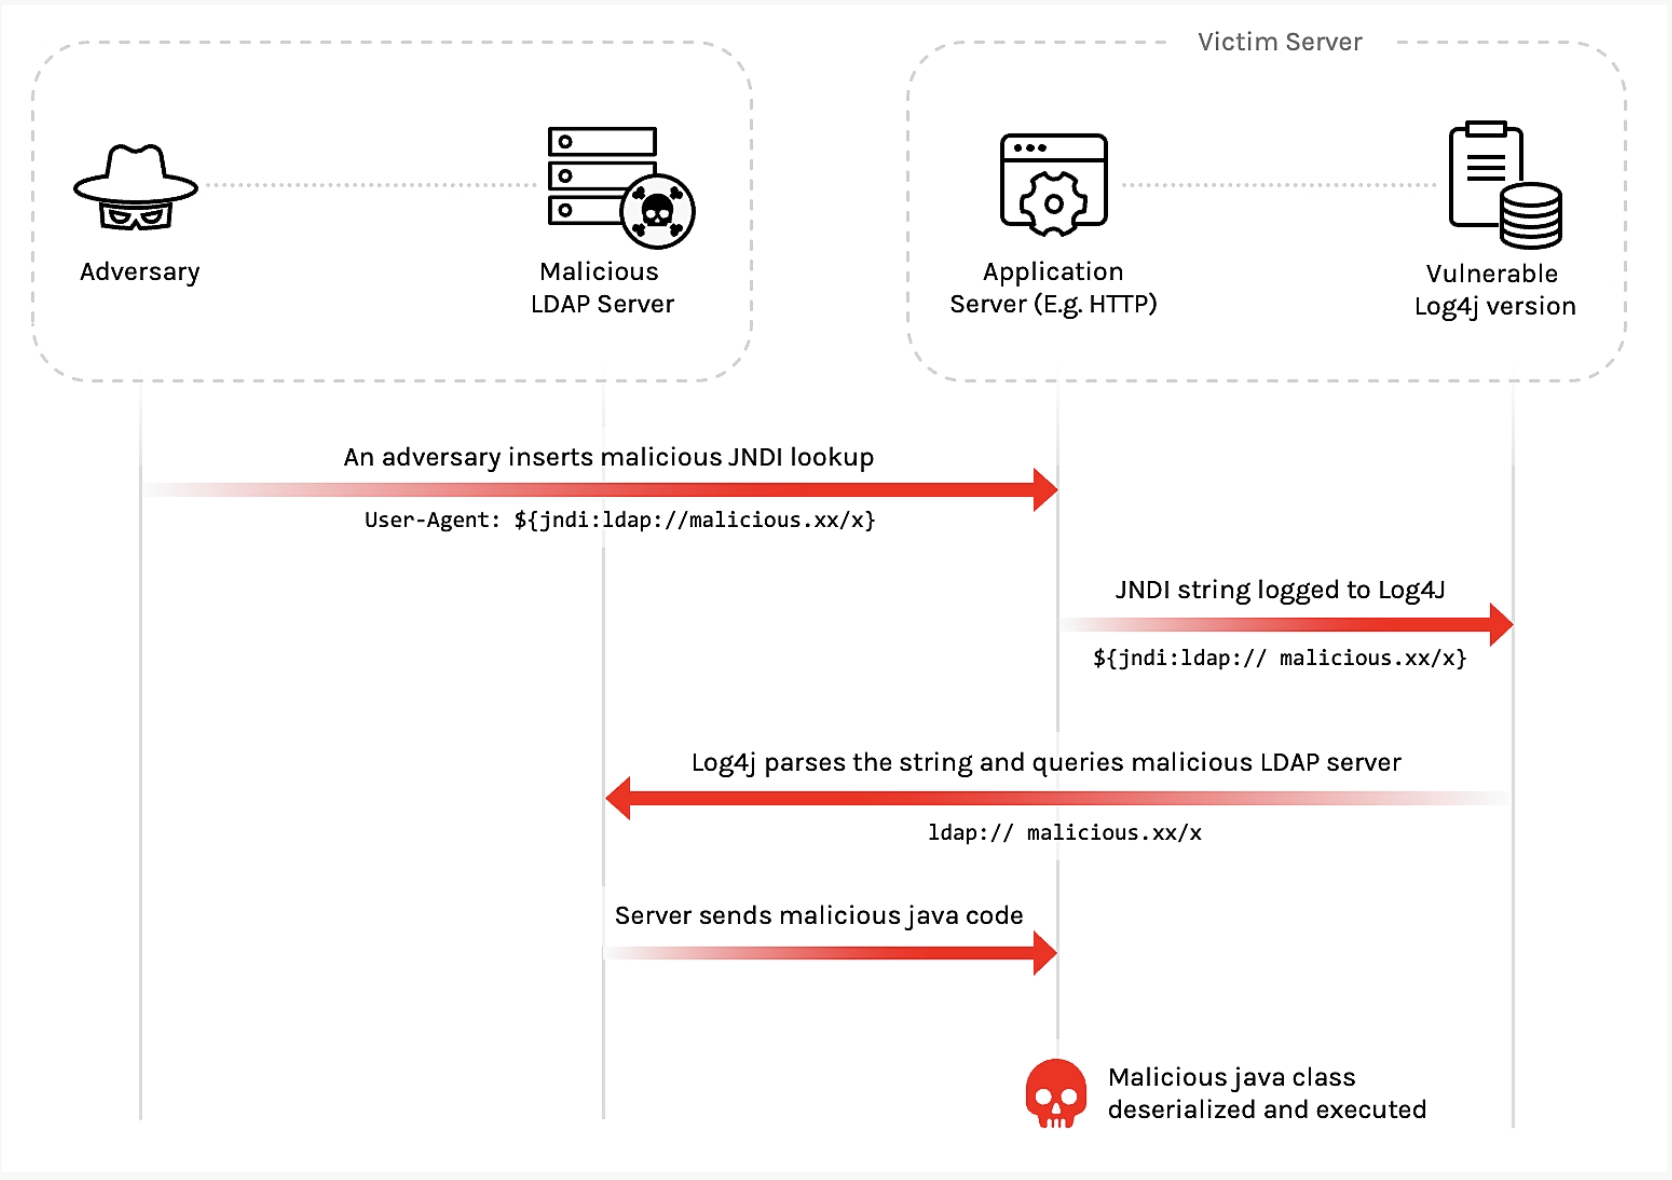
\includegraphics[width=0.50\textwidth]{LDAPAttack}
    \caption{Layout of the LDAP Attack on Log4j \cite{Holla}.}
    \label{fig:ldapAttack}
\end{figure}

Figure \ref{fig:ldapAttack} summarizes the attack that we conducted but we will go over the details
here. Versions of Log4j with the Log4Shell incorrectly handle Java Naming and Directory Interface (JNDI)
requests. JNDI requests are used as lookups for particular resources; these JNDI requests use URLs
that lead to a different server (such as an LDAP or DNS server) \cite{INCIBE}. Malevolent actors could 
thus set up their own server and then send a log message to a victim application server that uses a version 
of Log4j with the Log4Shell exploit. The log message sent by the attacker is a JNDI lookup that contains a URL
that directs the user to their server. Upon receiving this message, the application server has Log4j go 
through it. Upon performing the JNDI lookup, code from the attacker's own server is executed on the
victim server, leading to potentially catastrophic results \cite{Holla}. Depending on the attacker's motive,
the malicious code could cause anything from data leaks to server shutdowns.



\section{Related Work}
\label{sec:relatedWork}
While we did not do a full literature review of the material, the main article that inspired this investigation of 
ours was a set of experiments run by researchers Arreaga et al., in which they tested three different types 
of attacks (MITM, backdoor, and DoS) on a Raspberry Pi 3 Model B device with the Raspbian operating 
system. The researchers also performed the same suite of attacks on a VM that had the Windows 10 OS 
installed in order to compare the times for the attacks to be carried out. The goal of their research, like ours, 
was to highlight the major security flaws present in IoT devices, which are becoming more and more widely 
used. The authors note that with billions of IoT devices estimated to be in use by 2025, the opportunities for 
attackers to carry out devastating attacks against these devices (and thus the frameworks and systems they 
support) will only grow \cite{ARREAGA2023223}.

As for the results, the researchers were able to successfully execute all three attacks on both machines.
The total time to carry out the MITM and DoS attacks (which includes the setup and execution times) was
the same across both devices, but it was quicker to carry out the backdoor attack against the Raspberry Pi
than the Windows 10 VM. The authors note that the Raspberry Pi lacks "built-in virus and intrusion detection 
software," software which the Windows 10 VM had, making it relatively easier to attack the Pi. Their findings
highlight the treatment of security as a bonus feature or add-on with IoT devices, which (when considering the
widespread usage of these devices) can lead to disastrous consequences the likes of which no one has seen
before (including data breaches, service disruptions and shutdowns, and more). The authors recommend
some potential fixes to protect the Pi from these attacks, such as using a secure HTTPS protocol and limiting
traffic from a host, but they also warn about other potential attacks (such as DNS cache poisoning and
TCP sequence attacks) \cite{ARREAGA2023223}.




\section{Ethical Statement}

All attacks were performed only using machines owned and operated by the authors. The devices were connected to
CalPoly's eduroam network. However, no regular network traffic was disrupted, harmed, or observerd during any activities performed
over the course of this study. Additionally, the authors worked primarily to replicate known strategies for exploitation of a downpatched
Log4j, all of which have been fixed in any modern version of Java and the Log4j package from the last 5 years. 

\section{System Design}

This section offers description and details about our Raspberry Pi server configuration, attacker resources, and 
our specific exploit chain. Code for the main components of our setup and attack can be found in our archive, submitted
in tandem with this report. 

\subsection{SSH Hardening}

Prior to launching the Log4Shell attack, we took steps to close off easier avenues for attack on the Raspberry Pi, a
process commonly known as "server hardening". These steps are detailed from the tutorials followed, provided here [CITE HERE] and
here [CITE HERE]. However, we also offer brief description of the motivation behind these steps.

First and foremost, all SSH public keys of the authors were added to the authorized key list of the Pi. This allowed usage
to disable SSH Authentication via any means besides public key authentication. This is desireable due to the favorable 
security benefits offered by public key cryptography which are not present in the default, password-based login. Namely,
passwords are often crackable when configured lazily, phish from users, or present within known leaked password corpora. 
Our Raspberry Pi user credentials were no different, using the default username/password for a single sudo-enabled user.

The SSH port for the Raspberry Pi was also changed to 4707, away from the default of 22. This was done to prevent  
port scanner attacks, wherein common and default network ports on a machine are targetted by attackers for potential weakpoints.
Login as root was entirely disabled, instead opting to do all administrative tasks from our sudo-enabled user account. 
Full control when acting as the root user itself can be risky, and for our purposes it was never a necessary exposure.
Other server hardening tricks such as disabling outdated/insecure SSH protocols, firewalling, IP-banning, and whitelisting,
all of which are suggested in [CITE], were examined but not implemented on our server for the sake of time.

\subsection{Raspberry Pi Apache Server}

Apache2

Maven project

Springboot and Log4j

\subsection{Attacker Servers}

OpenLDAP

Inclusion of Java Schema

HTTP Server 

\subsection{Attack Execution}

Java Factory Exploit Object 

Process + attack. (Include image of the webpage with exploit string)

\section{Lessons Learned}

The dangers of Log4J, defenses provided to prevent our exploit chain. 

The struggles of downpatching Java. 

Resources on finding exploit strategies. Resources on finding (and trusting) exploit toolchains (i.e. the vulnerability testing repo).

\section{Conclusion}

\section{Acknowledgements}
The authors would like to thank Professor Stephen Beard for not only helping and directing us with this project
but also for making CSC-524 an all-around fun and interesting class to be in. This class would not have been
the same without him.



%%
%% The next two lines define the bibliography style to be used, and
%% the bibliography file.
\bibliographystyle{ACM-Reference-Format}
\bibliography{sample-base}


\end{document}
\endinput
%%
%% End of file `sigconf.tex'.
